\chapter{Spherical Glass Tonometer}\label{app:tonometer}

\begin{appbox}
	Back to Section~\ref{subsect:co2hb:pulse_carbametry:hb_prep}\hfill \hyperref[chapter:toc]{Main Table Of Content (TOC)}
\end{appbox}

The spherical glass tonometer used for the \gls{co2hb} spectrophotometry measurements related in Chapter~\ref{chap:co2hb} is depicted in Figure~\ref{annfig:tonometer:tonometer}, right. When used with the setup shown on the left-hand side of the figure, the rotation of the upper electric motor and the eccentric wheel agitates the tonometer in a manner similar to how one aerates red wine. This homogenises the haemolysate while maximising its exchange surface with the equilibration gas that flows over it, as depicted in the section view of the picture.

Of note, this piece of equipment has no specific name or serial number; it is a purely handcrafted contraption that has always belonged to the Orphy laboratory. As such, it may be compared with the tonometers used by Assendelft or Zijlstra, which are of a similar homemade nature\cite[Fig.~3.1]{assendelft1970}\cite[Fig.~6.1]{zijlstra2000}.

\begin{figure}
	\centering
	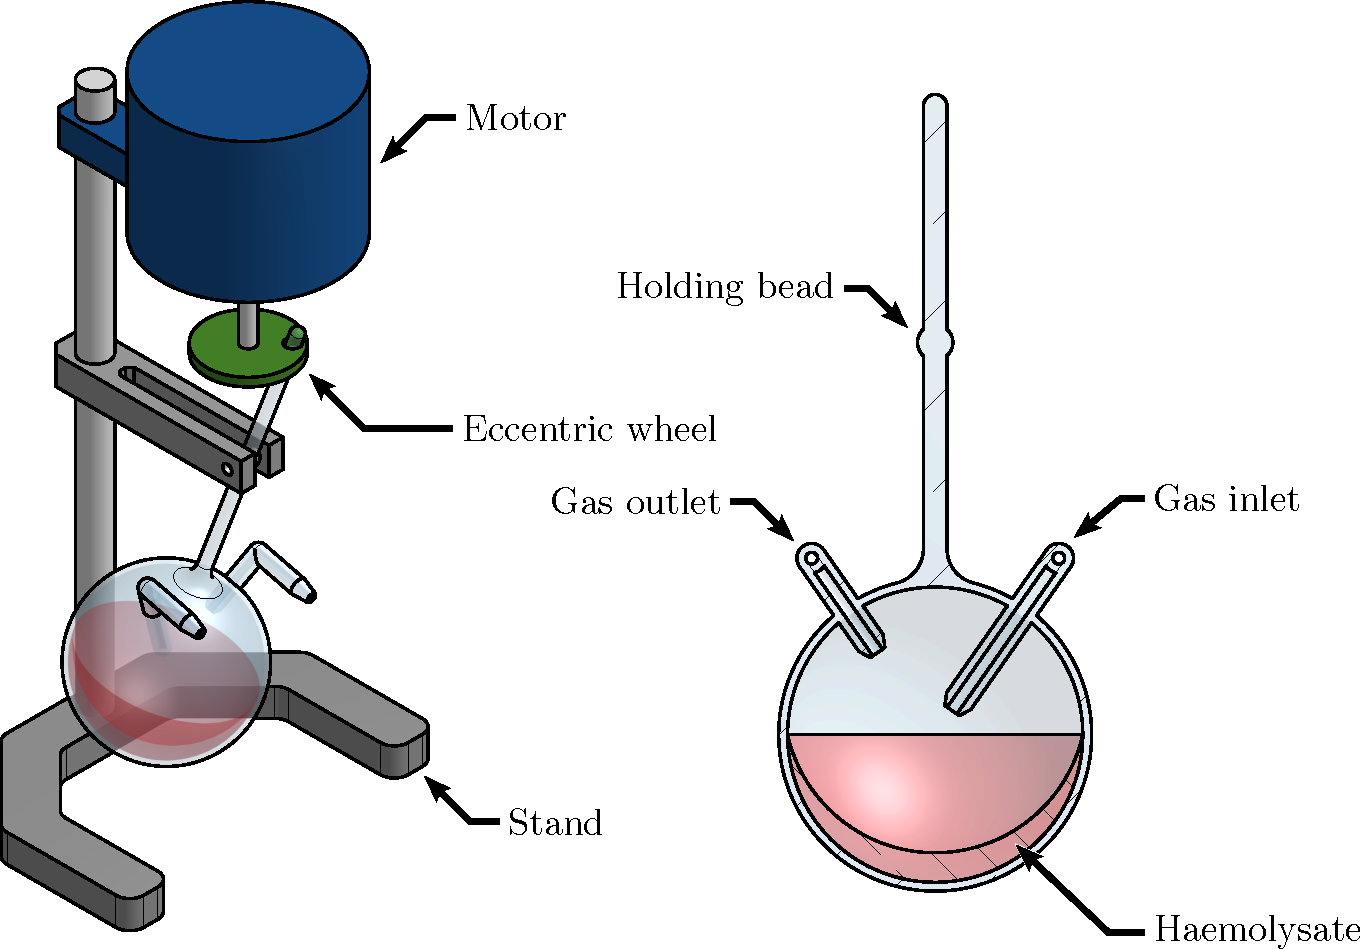
\includegraphics[width=\textwidth]{2_appendices/figures/tonometer.pdf}
	\caption[3D views of the spherical glass tonometer.]{\textbf{Left:} the whole tonometer assembly (inlet and outlet tubing not represented). \textbf{Right:} a section view of the spherical glass tonometer.}
	\label{annfig:tonometer:tonometer}
\end{figure}